\chapter{Introduction}

\emph{``There are only two hard things in Computer Science: cache invalidation and naming things.''} \vspace{-1cm}
\begin{flushright}-- Phil Karlton\end{flushright}

Web applications are becoming more and more dynamic with more personalized content that often requires complex data queries or computations based on large amounts of data. These computations can become a performance bottleneck in the application, which leads to slow response times and poor user experience for the users.

The performance can often be optimized by profiling and analyzing the code behind the computation, but it is often not the easiest solution, it does not guarantee a satisfactory performance in the end, and in some cases it is not possible to make the computation scale for large amounts of data. Caching is a popular solution for improving the performance and scalability in these cases, because it allows for a simple, scalable and generic way of addressing bottlenecks in the web applications.

Although it sounds like a silver bullet it also places a burden on the programmer that must locate and update the cached values while preserving consistency. The following description of an outage of the whole Facebook system, indicates the difficulty of cache management:

\begin{quote}
  The intent of the automated system is to check for configuration values that are invalid in the cache and replace them with updated values from the persistent store. This works well for a transient problem with the cache, but it doesn’t work when the persistent store is invalid.

 Today we made a change to the persistent copy of a configuration value that was interpreted as invalid. This meant that every single client saw the invalid value and attempted to fix it. Because the fix involves making a query to a cluster of databases, that cluster was quickly overwhelmed by hundreds of thousands of queries a second.
\begin{flushright}Robert Johnson~\cite{facebook_outage}\end{flushright}
\end{quote}

This example shows how critical the caching system can be and the importance of correctness.

This thesis will address this issue by reviewing the latest caching technique proposed in research and used in practice and contribute with a design and implementation of a open-source caching system in the Python programming language.

\section{Problem}
\label{sec:problem}

Most existing caching approaches are based on a pull based caching strategy, where cached values are updates as they are requested by the user, which leaves the user waiting for the cached value to be recomputed. The pull based caching strategy has the advantage that the system only stores cached values that are being requested, but the user requesting a cached value after it has been invalidated must wait for the computation to finish. In some cases, time taken to compute the cached values are finished within reasonable time, but in cases where the computation time exceeds the attention span of the user it becomes critical for the user experience. An alternative approach is to use an approach with a push-based strategy, where the system pre-computes the cached values so they are always served to the user directly from the cache.

Furthermore existing caching solutions leaves the responsibility for the programmer to manage the cache, which often leads to programming errors and makes caching difficult for the programmer to maintain.

These problems leads to the following challenges, which will be addressed by the thesis:

\textbf{Cache Management}

The first challenge related to cache management is faced in any caching system, where the programmer has to manage the caching system by naming the cached values and keeping them up to date such that the users are not presented with unexpected content.

One particular challenge within cache management is \emph{cache invalidation} that relies on the programmer correctly identifying every underlying data that affects the given cached value. The programmer then has to declare a way for the cached value to be invalidated when any of the underlying data changes. This analysis is difficult since it require global reasoning about how the underlying data changes in the application and which computations are being cached. Furthermore if the computation behind the cached value is altered to depend on new underlying data, the cache invalidation also has to change, making the cache prone to errors if the latter is forgotten.

We discuss this more in chapter~\ref{chapter:caching},~\ref{chapter:smache-cachable-functions}, and~\ref{chapter:invalidation}.

\textbf{Data Update Propagation}

The second challenge relates to the task of efficiently pre-computing the cached values, which easily becomes an expensive task for the system. To get around this the system must use an efficient technique for identifying when cached values updated and how to update them efficiently such that the cached values are ready for the users as soon as possible without using unnecessary CPU-power. This challenge will be addressed in chapter~\ref{chapter:data-update-propagation}.

% section problem end

\section{Requirements}
\label{sec:requirements}

The final solution addressing the problems described, will be designed with the following non-functional requirements:

\textbf{Software design:} Must be designed to be maintainable such that the programmer that uses the caching system understands how it works from using it and has the ability to extend it.

\textbf{Adaptability:} Should be convenient and easy to adapt into existing systems. This involves a flexible cache that can be extended to support multiple storage systems and cache databases.

\textbf{Efficiency:} Should be efficient with relation to performance such that it does not make existing operations of the systems significantly slower. It should also be efficient with relation to the system load such that it does not use more computational power than necessary to achieve the goal of the system.

\textbf{Scalability:} Should be designed for scalability in the sense that the design should still be efficient for large amount of data and applications deployed to multiple web servers working concurrently.

\textbf{Fault-Tolerance:} Should be designed with considerations on reliability, integrity and maintainability.

% section requirements end

\section{Context}
\label{sec:context}

To motivate the development and ensure the system is designed and implemented to be used in practive, the problem and requirements are based on a running web application - the Peergrade.io-platform.

\subsection{Peergrade.io Platform}
\label{subsec:the-peergrade-io-platform}

Peergrade.io is a platform for facilitating peer-evaluation in university and high school courses. Currently the platforms serves multiple institutions and thousands of students.

Universities and single teachers are able to sign up their courses to use Peergrade.io for facilitating peer-evaluation, where the students are able to grade and/or give each other feedback on their assignments. When a teacher has registered a course to use Peergrade.io, the teacher is able to create assignments. Beside the description of what the assignment is about, the teacher also sets deadlines for handing in and for the grading, and creates structured forms for the students to fill out with grades and text feedback.

When an assignment is open, the student is able to upload their hand-in. After the deadline for handing in is reached, the Peergrade.io platform will automatically distribute hand-ins for students to answer feedback questions and give grades. When the deadline for grading is reached, the feedback and grades are made available to the author of the hand-in, and the authors are able to indicate the helpfulness of the feedback by giving a constructive score or mark the feedback as inappropriate. After this step, the assignment is considered completed for the student. Figure~\ref{fig:student-screenshot} shows a screenshot of the Peergrade.io platform from the student's perspective.

\begin{figure*}[ht!]
  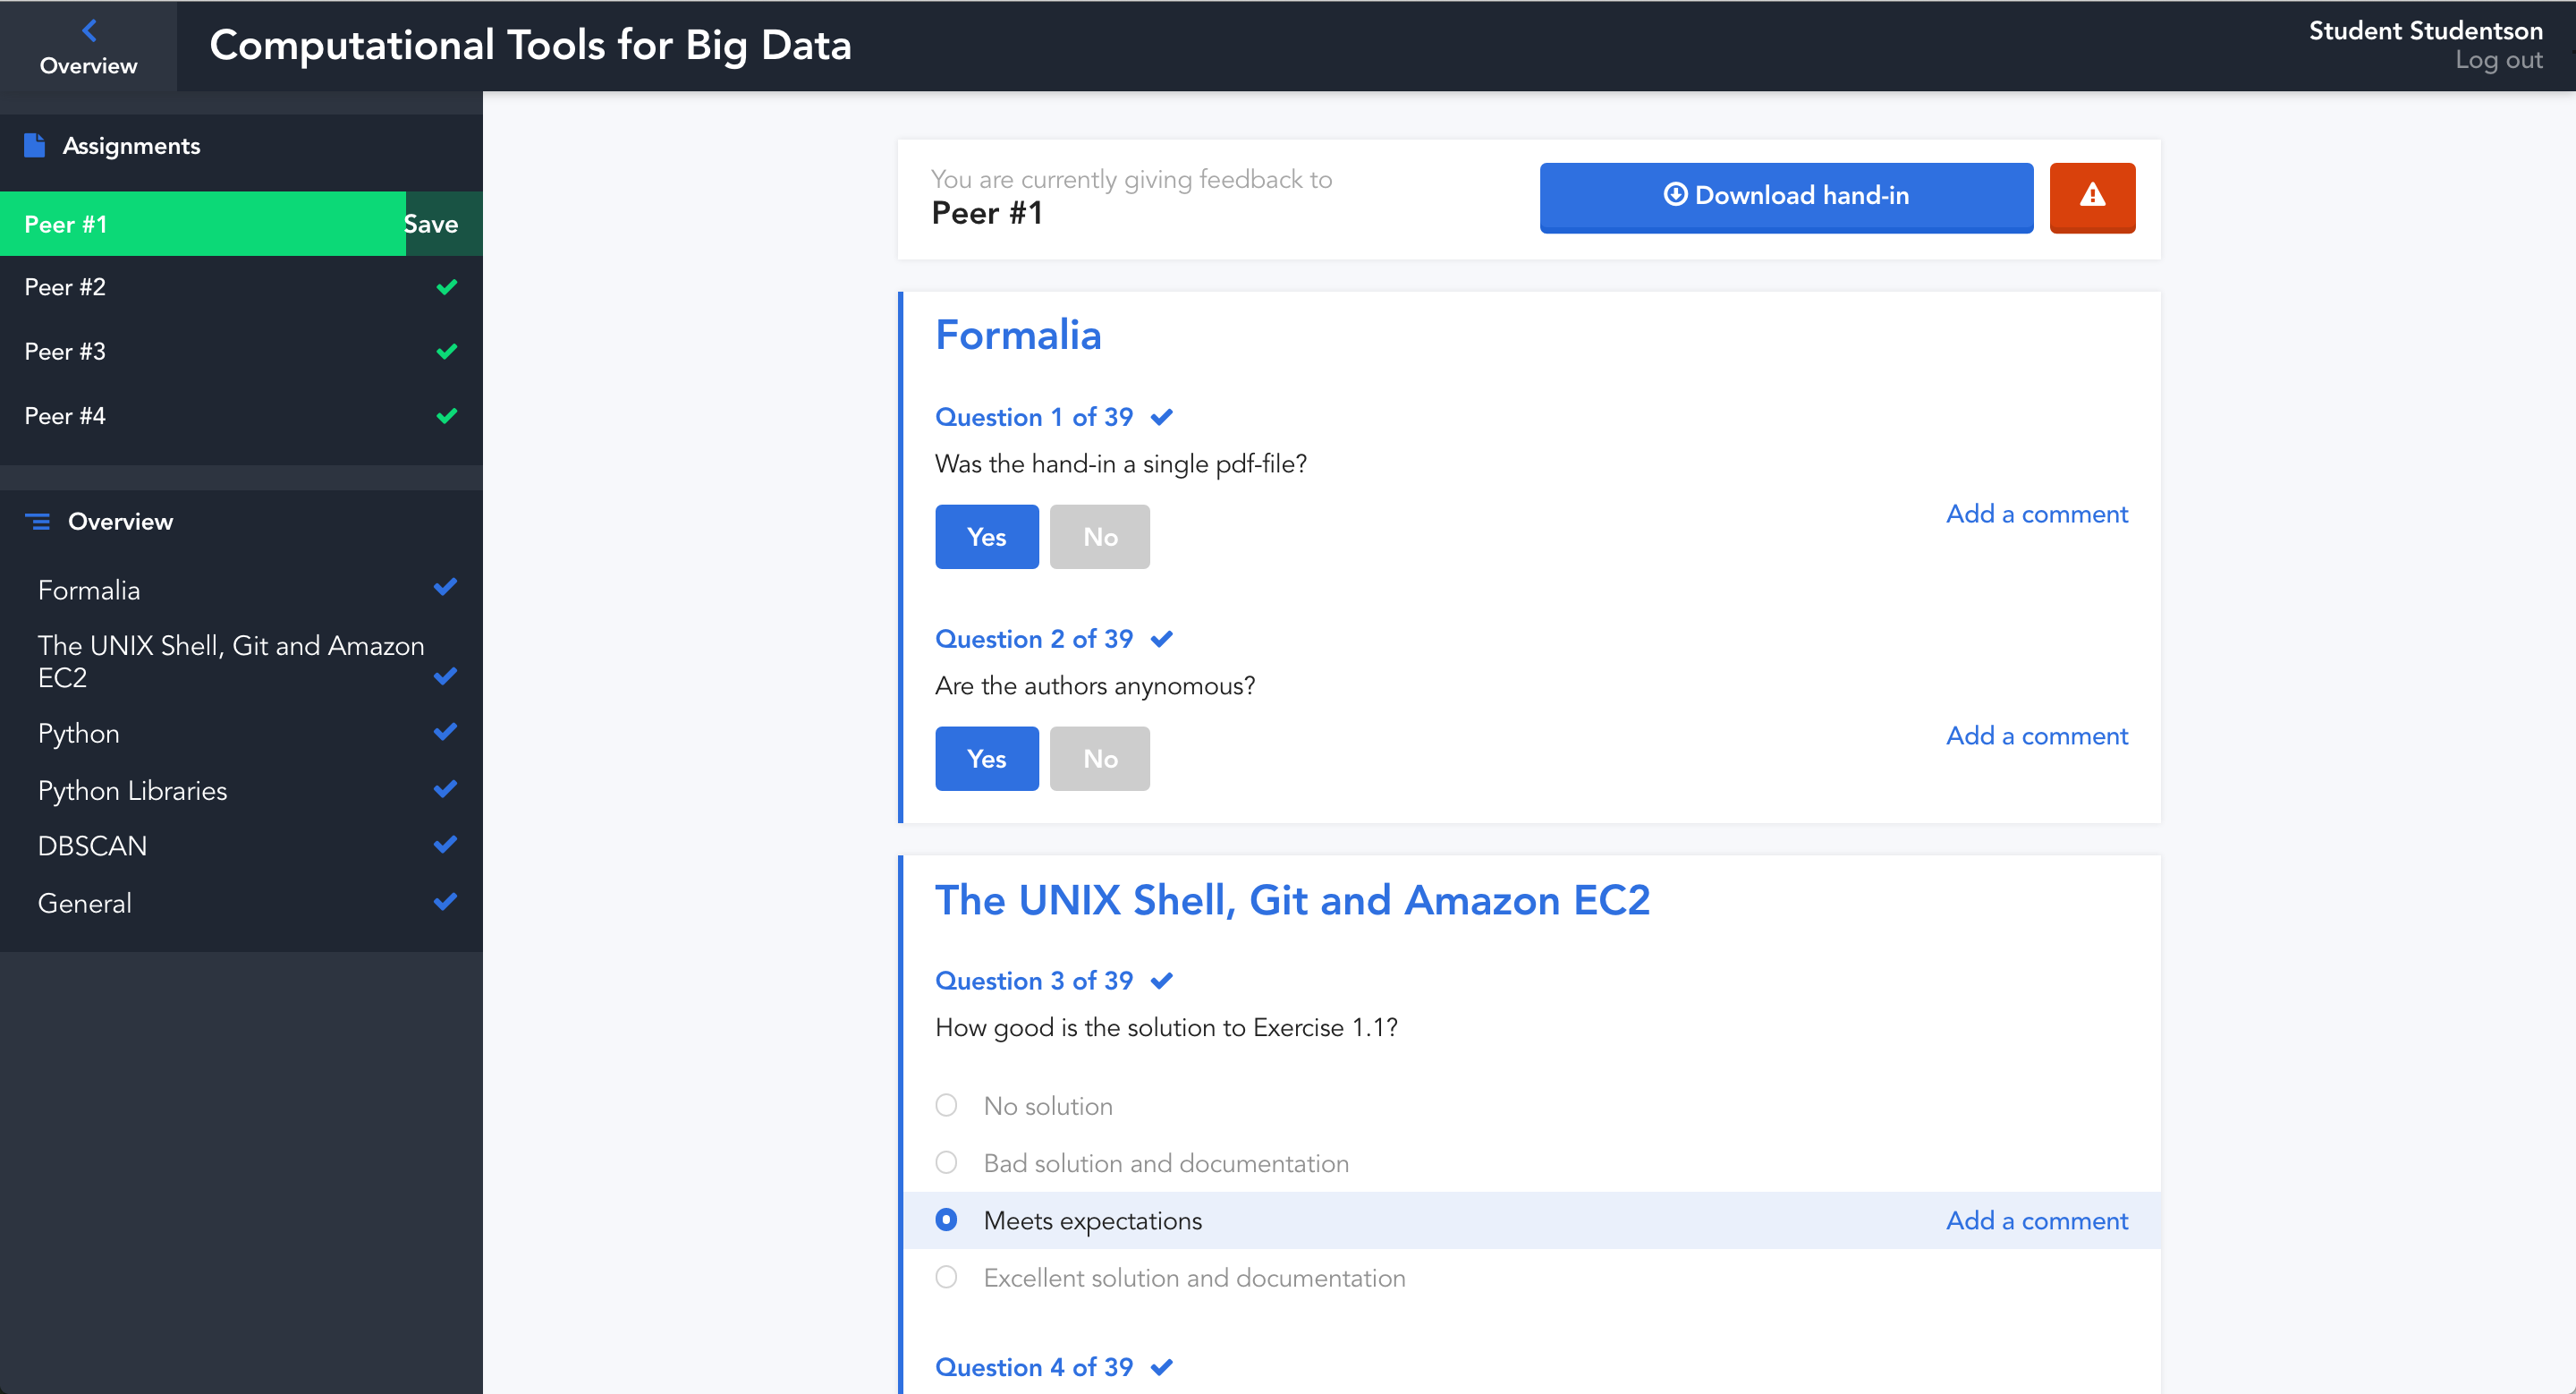
\includegraphics[width=\textwidth]{figures/screenshots/student_give_feedback.png}
  \caption[Screenshot from Peergrade.io]{A student grades another student's hand-in.}
  \label{fig:student-screenshot}
\end{figure*}

The last part of the platform is a complete overview of the assignment presented to the teacher with hand-ins, feedback, grades, constructive scores, and statistical analyses of to help the teachers assign grades. Furthermore the teacher is able to get a ``performance summary'' of a student to how the student performs compared to the rest of the participants. Figure~\ref{fig:teacher-screenshot} show screenshots of some of the interfaces seen by the teacher.

\begin{figure*}[ht!]
  \centering
  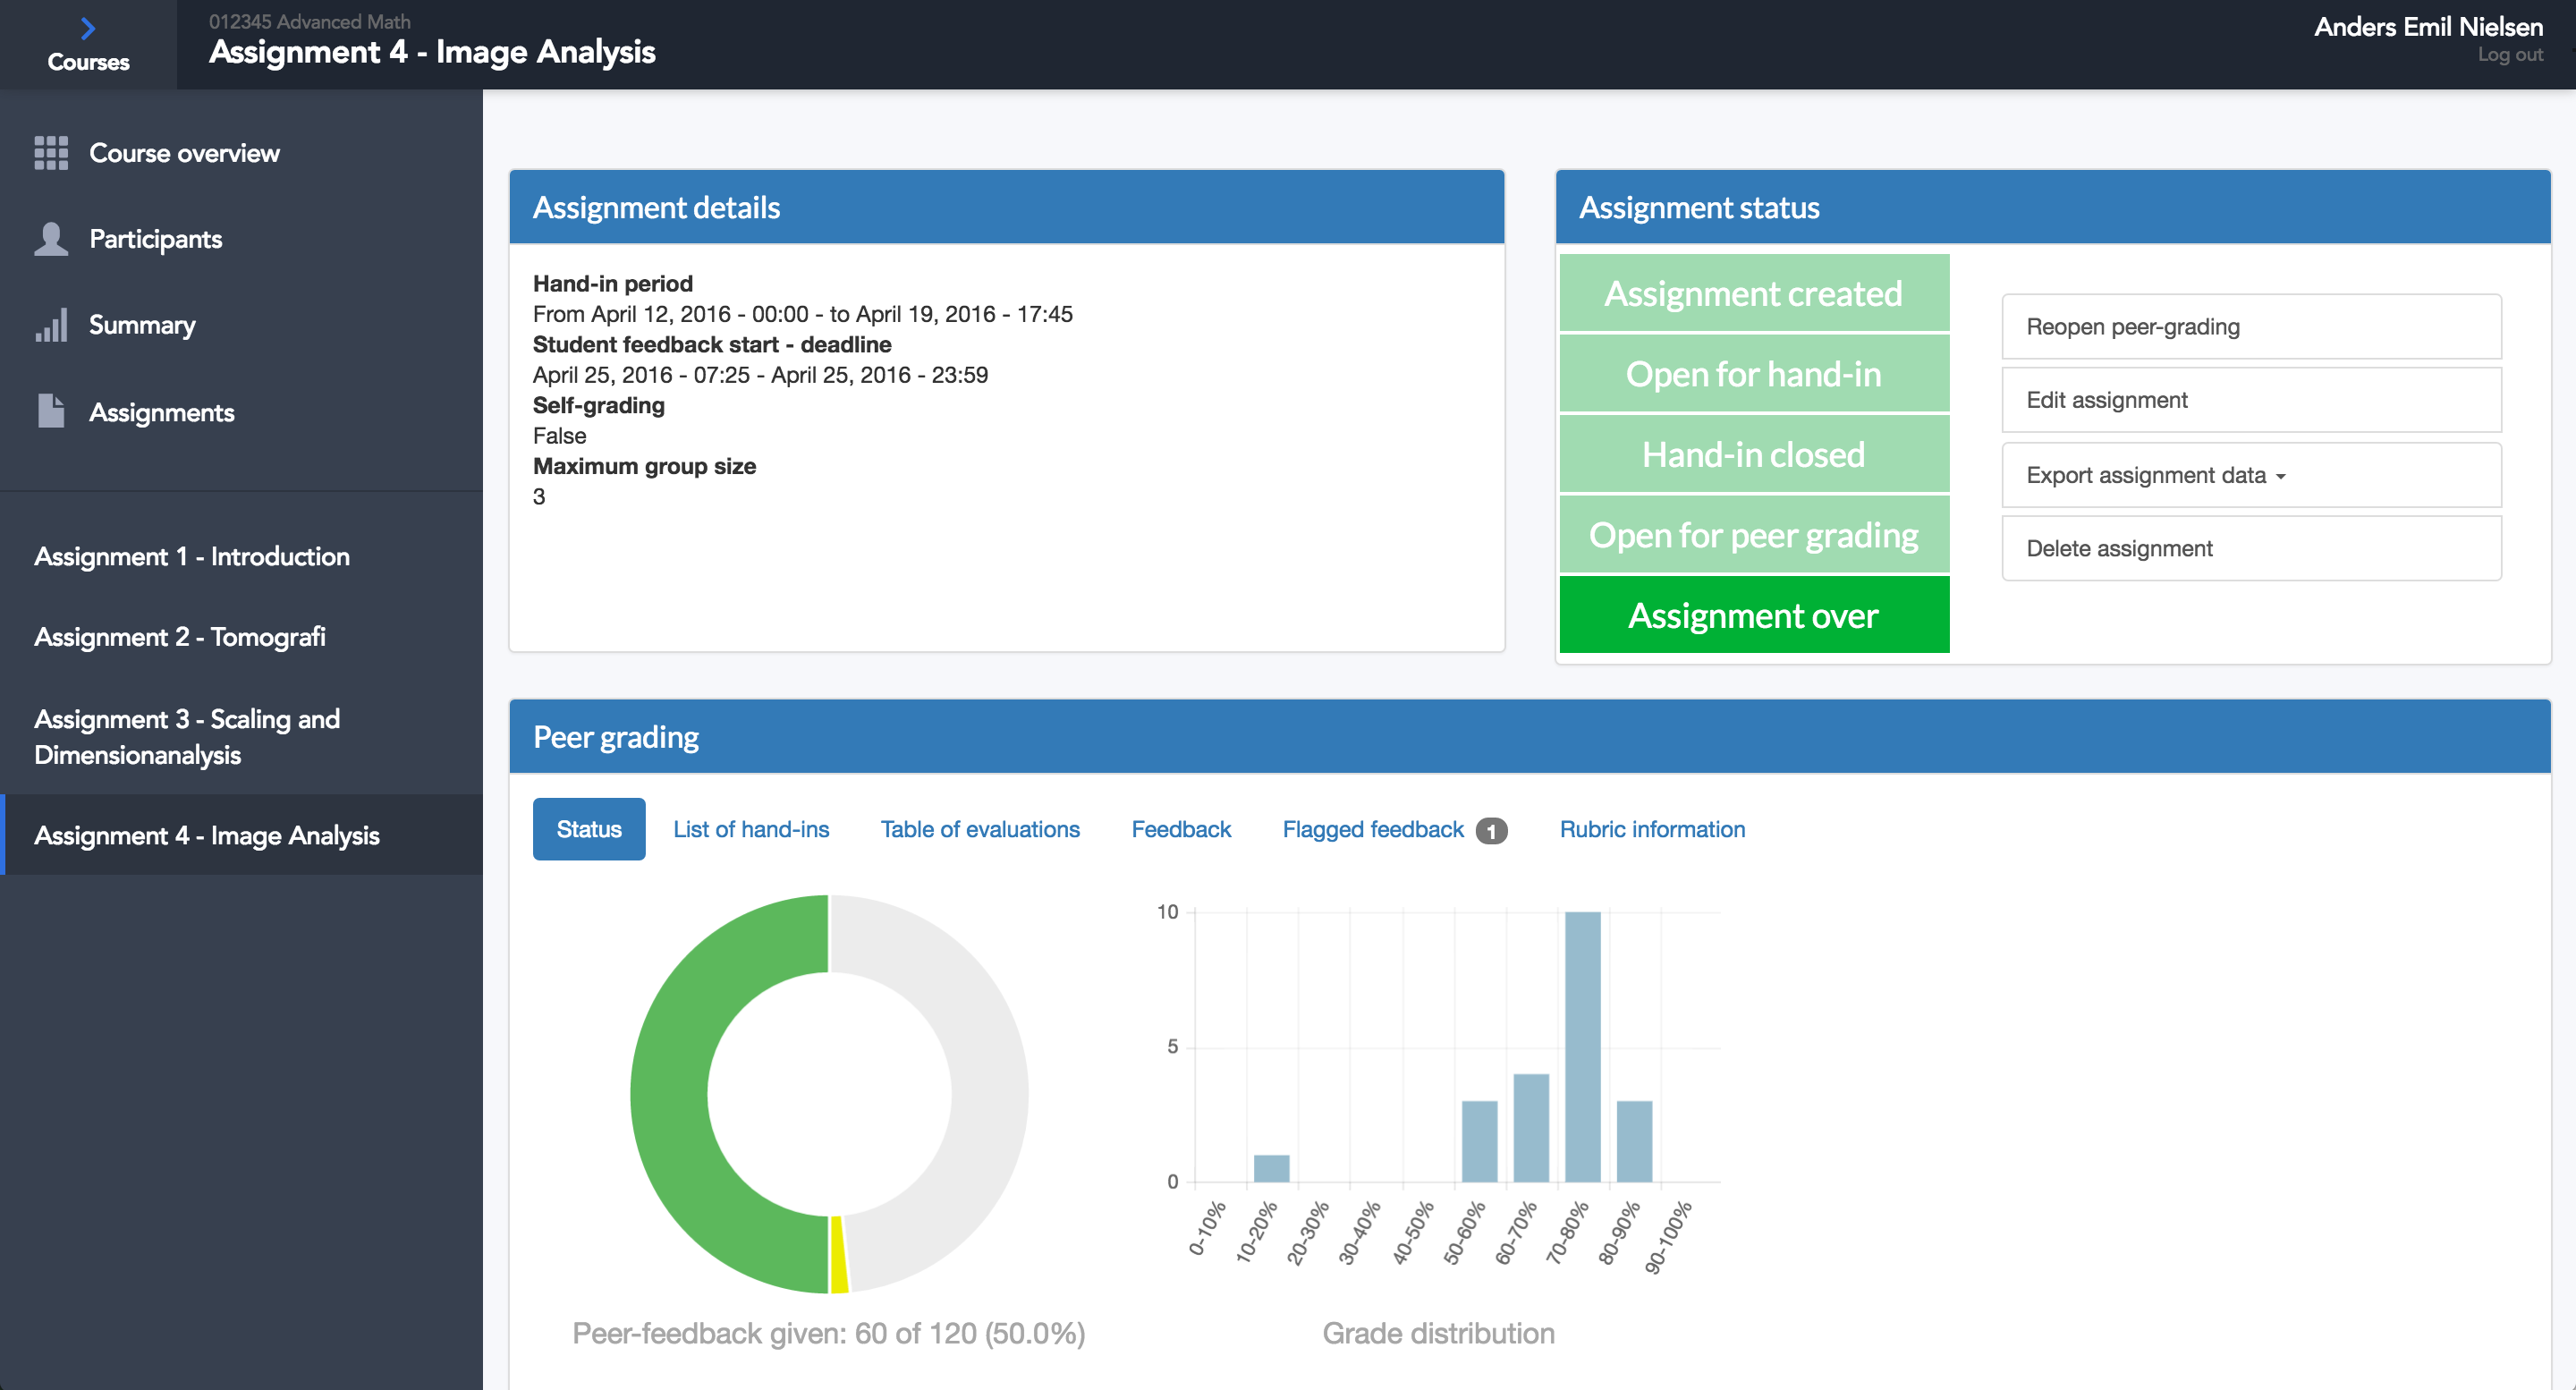
\includegraphics[width=1.0\linewidth]{figures/screenshots/teacher_assignment_overview.png}
  \caption[Screenshot from Peergrade.io]{A teacher sees the overview of a given assignment.}
  \label{fig:teacher-screenshot}
\end{figure*}

% subsection the-peergrade-io-platform end

\subsection{Running Example}
\label{subsec:running-example}

To relate the solution to a practical example, the thesis will use the running example seen in code snippet~\ref{code:running-example}.

\begin{code}{Code with the running example written in Python}
	\input{code/running_example.py}
	\label{code:running-example}
\end{code}

In this example we have a function \verb$course_score$ that computes the average score in a given course. To find the data for the participants the function makes a call to the primary storage, which returns a list of participant entities. The function iterates over these entities and calculates the participant score for a given participant using the function \verb$participant_score$. The function \verb$participant_score$ calls an external function that takes a long time to compute to illustrate a scenario related to the problem description. This example illustrates how the function \verb$course_score$ depends on the data for the course, participants, and grades given in the course. The same way we could say \verb$participant_score$ depends on the data for the given participant and the grades.

% subsection running-example end

% section context end

\section{Contributions}
\label{sec:contributions}

From the goal of finding and implementing a caching system that solves the problem in the context of the requirements described above, the thesis makes the following contributions.

First, we present a set of criteria used to evaluate caching approaches. These criteria are applied to existing approaches used in practical web development and proposed in research. The existing approaches are compared through an overview, which can be used to find a caching approach suitable for a given use case. By the end of the thesis the overview is extended with the solution proposed by this thesis, Smache.

Secondly, we present the design of Smache, a caching solution that aims to be easy to integrate into existing application and be able to cache the existing functions while invalidating and updating the cached values automatically. From this solution, the thesis makes the following technical contributions:

\begin{itemize}
  \item a \emph{programming model} that allows programmers to cache existing functions by declaring the dependencies to underlying data, after which the caching system automatically caches the result of the function by naming, localizing and storing the cached value for the function.
  \item a \emph{description and proof} of how to use \emph{timestamp invalidation} to invalidate and update cached values in a concurrent environment.
  \item an \emph{automatic invalidation system} based on \emph{timestamp invalidation} and a variant of a \emph{Simple Object Dependence Graph} for representing dependencies between cached values and underlying data.
  \item a \emph{data update propagation algorithm} based on \emph{timestamp invalidation} that is able to update all cached functions concurrently without additional concurrency control mechanisms.
\end{itemize}

Thirdly, we also present an implementation of Smache using the programming language Python, MongoDB as primary storage and Redis as the cache database, which is available open-source for future contributions at:

\url{https://github.com/anderslime/smache}

We have evaluated the performance and scalability of the data update propagation algorithm and how Smache affects existing operations on the application.

\section{Outline}
\label{sec:outline}

The overall structure of the thesis is as following:

With the motivation, problem, and requirements described in this introductory chapter, chapter~\ref{chapter:caching-model} will give an introduction to the basics of caching and explain the criteria used to evaluate caching approaches. Based on these criteria, existing caching approaches are compared in chapter~\ref{chapter:caching}. Chapter~\ref{chapter:smache-cachable-functions},~\ref{chapter:invalidation}, and~\ref{chapter:data-update-propagation} describes the solution suggested by this thesis by presenting the programming model that is then extended with automatic invalidation and afterwards with update on invalidation. Chapter~\ref{chapter:evaluation} covers experiments and evaluation of the final solution, and finally chapter~\ref{chapter:conclusion} lists the conclusions of the thesis.

In more detail, the different chapters covers the following subjects:

Chapter~\ref{chapter:caching-model} \emph{introduces caching} by presenting the basic caching algorithm, the common architecture of caching system, the models used to describe caching approaches, and \emph{criteria} used to evaluate caching approaches.

Chapter~\ref{chapter:caching} will \emph{describe and compare existing caching approaches} by applying the caching evaluation criteria.

Chapter~\ref{chapter:smache-cachable-functions} presents the overall solution of this thesis by describing the \emph{programming model} used to cache functions - cachable functions.

Chapter~\ref{chapter:invalidation} describes how cachable functions are extended with \emph{automatic invalidation} based on the \emph{Object Dependence graph} data structure and \emph{timestamp invalidation}.

Chapter~\ref{chapter:data-update-propagation} explains how the programming model is extended with update on invalidation using a data update propagation algorithm also based on \emph{timestamp invalidation}.

Chapter~\ref{chapter:evaluation} describes experiments performed to evaluate performance and efficiency, followed by an evaluation of Smache based on the results of the experiments and the requirements of the system.

Chapter~\ref{chapter:conclusion} finalize the thesis with a conclusion and suggestions for future work.

% section outline end


% section contributions end

